\documentclass[conference]{IEEEtran}

\usepackage{cite}
\usepackage{amsmath,amssymb}
\usepackage{graphicx}
\usepackage{booktabs}
\usepackage{array}
\usepackage{xcolor}
\usepackage{listings}
\usepackage{tikz}
\usepackage{url}
\usepackage{textcomp}
\usepackage[hidelinks]{hyperref}
\usetikzlibrary{positioning,arrows.meta,fit,backgrounds}

\graphicspath{{figures/}}

\lstset{
  language=Python,
  basicstyle=\ttfamily\scriptsize,
  keywordstyle=\bfseries,
  commentstyle=\itshape\color{gray},
  frame=single,
  rulecolor=\color{gray!60},
  breaklines=true,
  breakatwhitespace=false,
  columns=fullflexible,
  keepspaces=true,
  showstringspaces=false,
  xleftmargin=2pt,
  xrightmargin=2pt,
  aboveskip=4pt,
  belowskip=4pt
}

\newcommand{\code}[1]{\texttt{#1}}

\begin{document}

\title{Real-Time Stock Market Analysis of NASDAQ Equities Using Apache Kafka, Spark Structured Streaming and Spark MLlib}

\author{
\IEEEauthorblockN{Uttkarsh Ruparel}
\IEEEauthorblockA{PRN: 23070122227\\
Department of Computer Science and Engineering\\
Symbiosis Institute of Technology, Pune\\
Big Data Analytics (TE7552), CA-3}
\and
\IEEEauthorblockN{Dr. Akanksha Kulkarni}
\IEEEauthorblockA{Department of Computer Science and Engineering\\
Symbiosis Institute of Technology, Pune\\
Course Faculty}
}

\maketitle

\begin{abstract}
Equity markets emit one-minute bars for every listed company all day long, yet most student analyses of that data are run once, after the market has closed. This report presents a streaming pipeline that treats the same bars as an unbounded stream. One week of one-minute open-high-low-close-volume bars for 50 NASDAQ equities, 135,028 bars in total, is replayed in event-time order into Apache Kafka. Four Spark Structured Streaming queries consume the topic concurrently and compute validated raw bars, five-minute candles with volume-weighted average price, fifteen-minute sliding return volatility, and a per-bar anomaly score produced by a Spark MLlib KMeans model. Results are written to PostgreSQL and shown on a thirteen-panel Grafana dashboard. The anomaly model standardises every bar against the same symbol's statistics for the same half-hour of the trading day, so that the opening auction and the closing surge are not mistaken for anomalies. At a replay speed of 600 times real time the pipeline produced a median produce-to-process latency of 1.03 s and a 95th percentile of 1.93 s. All 27,249 candles agree exactly with an independent pandas computation. On a held-out session with 1\% injected anomalies, the KMeans detector reaches an area under the ROC curve of 0.968 against 0.862 for a univariate return z-score rule, and it is the only detector that notices volume-only events, although its F1 at the fixed threshold (0.50) is below the baseline (0.61). The report is explicit about its limits: the feed is a replay rather than a live exchange connection, the deployment is a single node, and the anomaly evaluation uses injected rather than labelled events.
\end{abstract}

\begin{IEEEkeywords}
Big Data analytics, Apache Kafka, Spark Structured Streaming, Spark MLlib, anomaly detection, NASDAQ, Grafana, PostgreSQL, real-time analytics
\end{IEEEkeywords}

\section{Introduction}

\subsection{Background and Motivation}
A listed company's share price is the output of thousands of buy and sell decisions made every second. Exchanges publish that activity at several granularities, and the one-minute bar is a common compromise: it keeps the opening price, the highest and lowest prices, the closing price and the traded volume of each minute. A single bar says very little. Fifty companies observed through a trading week, however, produce more than one hundred thousand bars, and the pattern across them describes how liquidity, risk and attention move through the market.

The usefulness of that description decays quickly. A volatility spike discovered the next morning cannot change the decision that was taken the previous afternoon. Operations teams that watch markets for risk or surveillance purposes therefore need the analysis to run as the data arrive. This is the classic setting for stream processing, in which a durable message log decouples the producers of events from the engines that analyse them, and the analysis is expressed as continuous queries over event time rather than as nightly jobs.

\subsection{Problem Statement}
The problem addressed is the following. Given a continuous stream of one-minute bars for a basket of NASDAQ equities, how can the bars be ingested, processed into windowed market indicators, scored for abnormal behaviour, stored and visualised within a few seconds of arrival using open-source Big Data tools, and how can the correctness of those results be demonstrated rather than assumed? The work does not attempt to generate trading signals or to predict prices. Its purpose is to build and document a working, verifiable, end-to-end reference pipeline whose design decisions are explained and whose outputs can be checked against the source data.

\subsection{Objectives}
The work pursued six measurable objectives:
\begin{enumerate}
\item acquire and validate one-minute bars for at least fifty NASDAQ symbols and document their schema;
\item ingest the bars into Apache Kafka in event-time order at a configurable replay speed;
\item compute five-minute candles with volume-weighted average price and fifteen-minute sliding volatility with Spark Structured Streaming, using event-time windows and watermarks;
\item train and serve a Spark MLlib anomaly detector inside the stream and compare it with a simple statistical baseline;
\item persist all outputs in PostgreSQL and present them on a Grafana dashboard; and
\item verify the streaming results against an independent computation and report throughput and latency honestly.
\end{enumerate}

\subsection{Scope and Contributions}
The scope is limited to descriptive analytics and anomaly detection on one-minute bars, executed on a single machine. Price prediction, order-book data, trading strategies and cluster deployment are outside the implemented system. The contributions are: (i) an architecture in which a timestamp-ordered replay stands in for a live feed while keeping event-time semantics intact; (ii) four concurrent streaming queries over one Kafka topic, each with its own checkpoint and a common metrics listener; (iii) a contextual anomaly model whose per-symbol, per-time-of-day baseline is joined to the stream as a static table, so that scoring needs no per-key state; (iv) an evaluation method that injects labelled anomalies into a held-out session and compares rankings by area under the curve as well as at a fixed threshold; and (v) an explicit cross-check of every windowed result against pandas.

\subsection{Organisation of the Report}
Section~II reviews the underlying concepts. Section~III states the requirements and environment. Sections~IV and V describe the dataset and the architecture. Sections~VI and VII document the streaming and machine learning implementations. Section~VIII presents results and visual insights, Section~IX reports testing and the problems met along the way, Section~X discusses the findings and limitations, and Section~XI concludes.

\section{Background and Related Work}

\subsection{Event Streaming with Apache Kafka}
Apache Kafka is a distributed, partitioned and replicated commit log \cite{kreps2011}. Producers append records to a named topic, and each topic is split into partitions that are individually ordered. Consumers read at their own pace and track their position as an offset, so a slow consumer never blocks a fast producer and several consumers can read the same history independently. Records that share a key are routed to the same partition, which gives per-key ordering. Recent Kafka releases run without ZooKeeper in the KRaft mode, in which the brokers manage their own metadata quorum \cite{kip500}; this simplifies a single-machine deployment to one container.

\subsection{Spark Structured Streaming}
Apache Spark generalised MapReduce with in-memory working sets and resilient distributed datasets \cite{zaharia2010,zaharia2012}. Structured Streaming exposes a stream as an unbounded table and lets the same DataFrame operations run incrementally \cite{armbrust2018}. Two ideas matter for this project. First, aggregation is defined over event time, the time recorded in the data, rather than over the time a record happens to arrive. Second, a watermark tells the engine how late data may be, so that it can finalise a window, emit it once in append mode and discard its state. These ideas follow the dataflow model, which separates what is computed from when results are materialised \cite{akidau2015}.

\subsection{MLlib and KMeans Clustering}
MLlib is Spark's distributed machine learning library \cite{meng2016}. Its KMeans estimator implements Lloyd's iterative algorithm \cite{lloyd1982} and, by default, the parallel k-means$\|$ initialisation, a scalable variant of k-means++ seeding \cite{arthur2007,bahmani2012}. A fitted model can be placed in a \code{Pipeline} with a feature assembler and applied to a streaming DataFrame with \code{transform}, which is how the model is served in this work.

\subsection{Anomaly Detection in Market Data}
Anomaly detection techniques are surveyed by Chandola \emph{et al.}\ \cite{chandola2009}, who distinguish point anomalies from \emph{contextual} anomalies, which are abnormal only relative to a context. Intraday market data are a clear case of the latter. Trading volume and price variability are known to follow a pronounced pattern across the trading day, high at the open, low at midday and rising again towards the close \cite{admati1988}. A bar with twice the average volume is unremarkable at 09:30 and remarkable at 12:30. A detector that ignores the time of day will flag every opening minute and miss the genuinely unusual midday events, which is why this work normalises each bar against its own context.

\subsection{Storage and Visualisation}
PostgreSQL provides indexed SQL aggregation for the volumes involved here, and Grafana can query it directly and present time series, candlesticks, bar charts and status grids in one dashboard \cite{pgdocs,grafanadocs}. Kafka is used as the transport rather than as the store of record, which is the pattern recommended for data-intensive systems \cite{kleppmann2017}.

\subsection{Alternatives and Design Rationale}
Apache Flink \cite{carbone2015} and Kafka Streams are capable stream processors and were considered. Spark was chosen because the course emphasises it, because MLlib lets the model and the stream live in one engine and one language, and because the micro-batch trigger gives a latency of one to two seconds, which is adequate for one-minute bars. Elasticsearch with Kibana was not chosen because the questions asked are relational aggregations by symbol and window, which PostgreSQL expresses in a few lines. Predicting whether the next bar will close up or down was rejected as the machine learning task because one-minute returns are close to unpredictable and a classifier would hover around fifty per cent accuracy; anomaly detection is a more defensible and more useful task for a monitoring system.

\subsection{Gap Addressed}
Introductory market projects commonly show either a batch notebook over historical prices or a toy producer that sends random numbers. This work sits between the two. It streams real market bars through a production-grade message log, applies event-time windowing with watermarks, serves a trained model inside the stream, and subjects the result to verification and evaluation, while stating plainly what a replay on one machine can and cannot show.

\section{Requirements and Methodology}

\subsection{Functional Requirements}
\begin{enumerate}
\item FR1: acquire one-minute OHLCV bars for at least fifty NASDAQ symbols and store them in a re-usable cache.
\item FR2: publish the bars to Kafka keyed by symbol, in event-time order, at a configurable speed.
\item FR3: compute five-minute candles, volume-weighted average price and fifteen-minute sliding volatility using event-time windows.
\item FR4: score every bar with a trained anomaly model and flag abnormal bars.
\item FR5: store all results in a relational database and expose them to a dashboard.
\item FR6: record pipeline throughput and latency so that performance can be inspected.
\end{enumerate}

\subsection{Non-Functional Requirements}
The pipeline should deliver a result within five seconds of a bar being published, run within the 16~GB of memory of the development laptop, resume from its checkpoints after a restart without duplicating rows, and be reproducible from a clean checkout with a small number of commands. Code is expected to be formatted and to pass static linting.

\subsection{Environment}
Table~\ref{tab:env} lists the software environment. Versions are those reported by the tools in the terminal sessions or pinned in the project files.

\begin{table}[t]
\caption{Software and Hardware Environment}
\label{tab:env}
\centering
\small
\begin{tabular}{@{}p{3.3cm}p{4.9cm}@{}}
\toprule
Component & Version / setting \\
\midrule
Machine & MacBook Air, 16~GB RAM, macOS \\
Java & OpenJDK 17.0.20 \\
Python & 3.12.10 \\
Apache Spark (PySpark) & 4.0.4, local mode, \code{local[*]} \\
Apache Kafka & 3.9.0, KRaft, single broker \\
PostgreSQL & 16 (Alpine image), JDBC 42.7.4 \\
Grafana & 11.3.0 \\
Kafka UI & 0.7.2 \\
confluent-kafka & 2.16.0 \\
yfinance & 1.7.0 \\
Docker / Compose & 29.4.1 / 5.1.3 \\
Docker VM memory & 11.7~GiB \\
\bottomrule
\end{tabular}
\end{table}

\subsection{Workflow}
The work followed six stages. Bars were first downloaded and validated. A Kafka broker, PostgreSQL and Grafana were then started with Docker Compose. A replay producer was written and tested against the topic. The Spark queries were developed next and checked on a drained backlog before being run live. The anomaly model was trained offline, evaluated and added to the stream. Finally, the dashboard was provisioned from files and the whole system was verified and measured.

\section{Dataset and Data Preparation}

\subsection{Origin and Structure}
The data are one-minute bars obtained through the \code{yfinance} library \cite{yfinance} for 50 large NASDAQ-listed companies (the list is in Appendix~C). The request covered the most recent seven calendar days, which yielded seven regular trading sessions from 1 to 9 October 2026 (the library serves one-minute history for roughly the last week only). Table~\ref{tab:schema} gives the schema, which is kept identical from the Parquet cache through Kafka to the first PostgreSQL table.

\begin{table}[t]
\caption{Bar Schema}
\label{tab:schema}
\centering
\small
\begin{tabular}{@{}p{2.55cm}p{1.9cm}p{3.5cm}@{}}
\toprule
Field & Type & Meaning \\
\midrule
\code{symbol} & string & Ticker; also the Kafka key \\
\code{bar\_time} & timestamp (UTC) & Start of the one-minute bar \\
\code{open}, \code{high}, \code{low}, \code{close} & double & Prices in US dollars \\
\code{volume} & long & Shares traded in the minute \\
\bottomrule
\end{tabular}
\end{table}

\subsection{Validation}
Table~\ref{tab:quality} records the checks applied to the cached data. The bars contain no missing values and no duplicate symbol and minute pairs, and the price relations are internally consistent. A symbol has between 2,387 and 2,729 bars against a theoretical 2,730 (seven sessions of 390 minutes), because some minutes have no recorded bar; the replay preserves these gaps rather than filling them.

\begin{table}[t]
\caption{Data Quality Checks on the Cached Bars}
\label{tab:quality}
\centering
\small
\begin{tabular}{@{}lr@{}}
\toprule
Check & Result \\
\midrule
Rows & 135,028 \\
Symbols & 50 \\
Trading sessions & 7 \\
Null values & 0 \\
Duplicate (symbol, minute) pairs & 0 \\
Bars with high $<$ low & 0 \\
Bars with high $<$ max(open, close) & 0 \\
Bars with low $>$ min(open, close) & 0 \\
Bars with non-positive open & 0 \\
Zero-volume bars & 12 \\
Close price range (USD) & 20.50 -- 1,891.58 \\
Total shares traded & 3.92 billion \\
\bottomrule
\end{tabular}
\end{table}

\subsection{Cleaning and Preparation}
Rows are retained only if the open price is positive and the high is not below the low. Prices are rounded to four decimal places because the source returns single-precision values whose binary representation otherwise leaks into the output as digits such as 245.3699951171875. Timestamps are converted to UTC and stored with microsecond precision, which is the resolution Spark reads from Parquet without conversion. A failure of one symbol in the multi-threaded download, caused by a lock on the library's local time-zone cache, is handled by retrying missing symbols sequentially, so every run returns all fifty.

\subsection{Timestamp Rebasing}
A market is open for only 6.5 hours of each weekday and the history served by the data source is short, so a dashboard with a relative time range such as ``last three days'' would silently empty as the cached data aged. The producer therefore shifts all timestamps by a whole number of days so that the final session falls on the previous calendar day. A whole-day shift preserves the time of day, the weekend gap and every relationship between bars, which are the properties the analytics depend on. In the run reported here the shift was one day, so source sessions 1--9 October appear as 2--10 October in the database. Event times in the report are quoted on the replayed calendar unless stated otherwise.

\subsection{Limitations of the Data}
The data are a one-week sample at one-minute resolution, so seasonal patterns beyond the intraday cycle cannot be studied. The source is an unofficial interface and offers no service guarantee. The bars are adjusted for splits and dividends by the library, and corporate-action events are not modelled. Finally, the replay is historical: it exercises the system faithfully but it is not a live exchange connection.

\section{System Architecture}
Fig.~\ref{fig:arch} shows the end-to-end design. Bars flow left to right and top to bottom. The replay producer publishes JSON messages to the \code{ticks.raw} topic. Four Spark queries read that topic independently, each with its own consumer offsets and checkpoint, and each writes one PostgreSQL table through a \code{foreachBatch} sink. A listener attached to the Spark session writes one metrics row per micro-batch, and Grafana reads the tables with SQL.

\begin{figure*}[t]
\centering
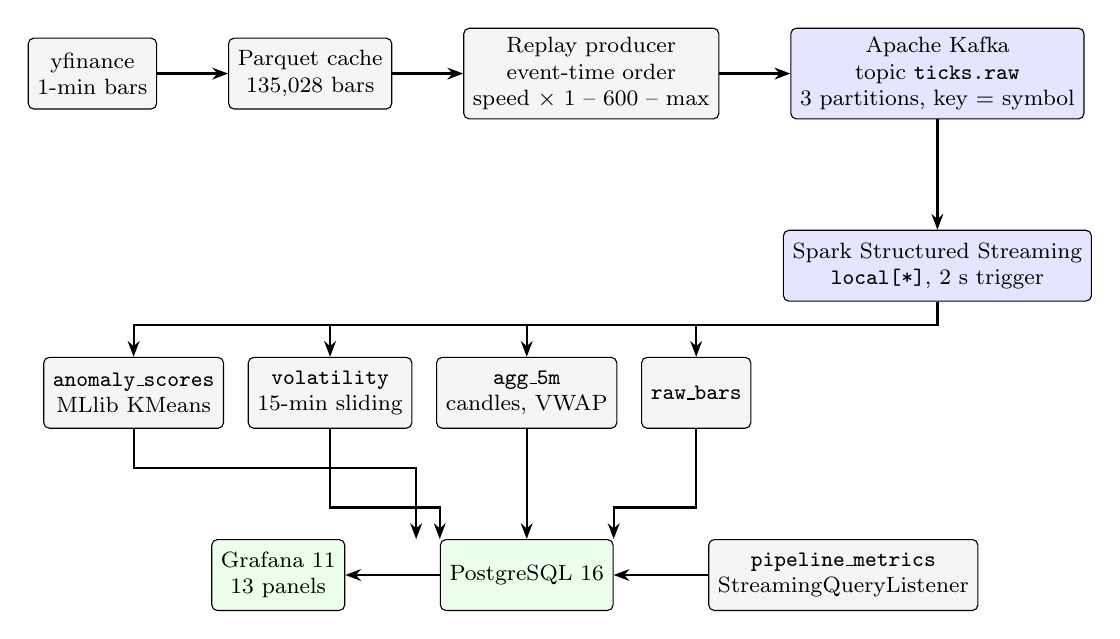
\begin{tikzpicture}[
  node distance=7mm and 9mm,
  box/.style={draw, rounded corners=2pt, minimum height=9mm, align=center, font=\footnotesize, fill=gray!8},
  strong/.style={box, fill=blue!10},
  sink/.style={box, fill=green!8},
  flow/.style={-{Stealth[length=2mm]}, thick}
]
\node[box] (yf) {yfinance\\1-min bars};
\node[box, right=of yf] (cache) {Parquet cache\\135,028 bars};
\node[box, right=of cache] (prod) {Replay producer\\event-time order\\speed $\times$ 1 -- 600 -- max};
\node[strong, right=of prod] (kafka) {Apache Kafka\\topic \code{ticks.raw}\\3 partitions, key = symbol};
\node[strong, below=14mm of kafka] (spark) {Spark Structured Streaming\\\code{local[*]}, 2~s trigger};
\node[box, below left=7mm and 4mm of spark] (q1) {\code{raw\_bars}};
\node[box, left=3mm of q1] (q2) {\code{agg\_5m}\\candles, VWAP};
\node[box, left=3mm of q2] (q3) {\code{volatility}\\15-min sliding};
\node[box, left=3mm of q3] (q4) {\code{anomaly\_scores}\\MLlib KMeans};
\node[sink, below=14mm of q2] (pg) {PostgreSQL 16};
\node[sink, left=12mm of pg] (gf) {Grafana 11\\13 panels};
\node[box, right=12mm of pg] (met) {\code{pipeline\_metrics}\\StreamingQueryListener};
\draw[flow] (yf) -- (cache);
\draw[flow] (cache) -- (prod);
\draw[flow] (prod) -- (kafka);
\draw[flow] (kafka) -- (spark);
\draw[flow] (spark.south) -- ++(0,-3mm) -| (q1.north);
\draw[flow] (spark.south) -- ++(0,-3mm) -| (q2.north);
\draw[flow] (spark.south) -- ++(0,-3mm) -| (q3.north);
\draw[flow] (spark.south) -- ++(0,-3mm) -| (q4.north);
\draw[flow] (q1.south) |- ([yshift=4mm]pg.north east) -- (pg.north east);
\draw[flow] (q2.south) -- (pg.north);
\draw[flow] (q3.south) |- ([yshift=4mm]pg.north west) -- (pg.north west);
\draw[flow] (q4.south) -- ++(0,-5mm) -| ([xshift=-3mm]pg.north west);
\draw[flow] (met) -- (pg);
\draw[flow] (pg) -- (gf);
\end{tikzpicture}
\caption{End-to-end architecture of the streaming pipeline.}
\label{fig:arch}
\end{figure*}

Table~\ref{tab:tables} lists the PostgreSQL tables and their grain. Raw bars are retained so that every aggregate can be recomputed and audited, and the anomaly table carries the model's intermediate z-scores so that a flag can be explained after the fact.

\begin{table}[t]
\caption{PostgreSQL Tables Written by the Pipeline}
\label{tab:tables}
\centering
\small
\begin{tabular}{@{}p{2.7cm}p{3.7cm}r@{}}
\toprule
Table & Grain & Rows \\
\midrule
\code{raw\_bars} & one bar per symbol per minute & 135,028 \\
\code{agg\_5m} & symbol and five-minute window & 27,249 \\
\code{volatility} & symbol and sliding 15-minute window & 140,550 \\
\code{anomaly\_scores} & one scored bar & 135,028 \\
\code{pipeline\_metrics} & query and micro-batch & 567 \\
\bottomrule
\end{tabular}
\end{table}

\section{Streaming Implementation}

\subsection{Kafka Broker and Topic}
A single Kafka 3.9 broker runs in KRaft mode in a container. Two listeners are exposed, one for clients on the host and one for containers on the Docker network, so that both the Python producer and the Kafka UI container can connect. The producer creates the topic \code{ticks.raw} if it is missing, with three partitions and a replication factor of one. Keying messages by symbol means that all bars of a company land on one partition in order. Fig.~\ref{fig:kafka} shows the topic after a partial replay; the three partitions hold unequal counts because fifty keys do not hash evenly over three partitions.

\begin{figure}[t]
\centering
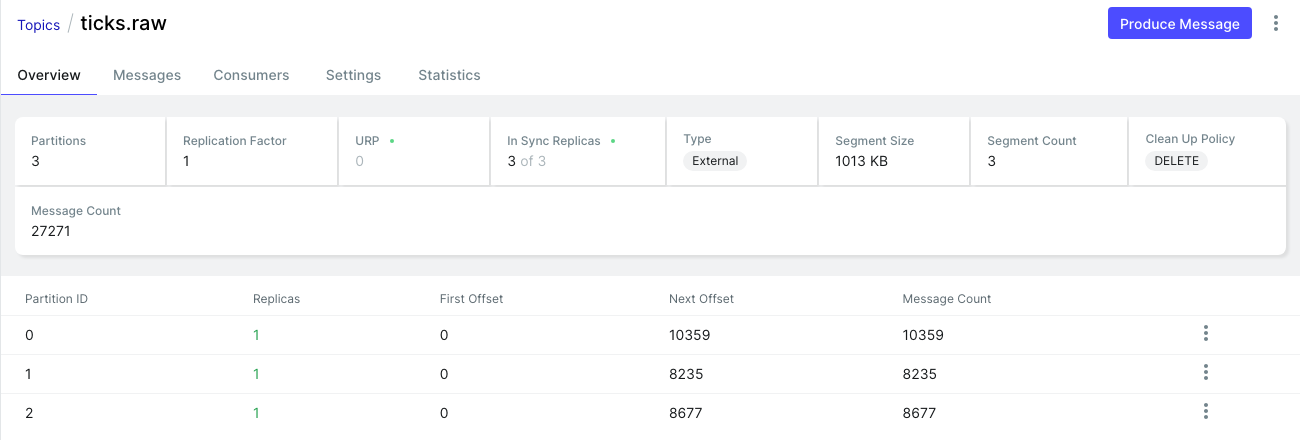
\includegraphics[width=\columnwidth]{fig_kafka_topic.png}
\caption{Topic \code{ticks.raw} in Kafka UI during a replay: three partitions, per-partition offsets and the message count.}
\label{fig:kafka}
\end{figure}

\subsection{Replay Producer}
The producer reads the Parquet cache, sorts by timestamp and symbol, and groups the rows by timestamp. Each group is one market minute. After sending a group it sleeps for $60/S$ seconds, where $S$ is the speed multiplier, so $S=60$ sends one market minute per second and $S=0$ removes the pause entirely. Overnight and weekend gaps are skipped rather than waited for, so a whole week of 2,730 distinct minutes takes about 4.5 minutes at $S=600$. The producer uses idempotent delivery with \code{acks=all}, LZ4 compression and a 20~ms linger, and it counts delivery callbacks so that a failed message is reported rather than lost. In an unthrottled run it delivered all 135,028 messages in 1.4 s, about 95,000 messages per second, which shows that the producer is not the bottleneck.

\subsection{Ingestion and Parsing in Spark}
Each query subscribes to the topic, reads from the earliest offset with at most 20,000 records per trigger, and parses the JSON value with an explicit schema. The text timestamp is converted to a timestamp type, and two further columns are kept for observability: \code{kafka\_time}, the timestamp stamped on the message by the producer client, and \code{processed\_time}, the time Spark evaluated the micro-batch. Their difference is the produce-to-process latency reported in Section~VIII.

\subsection{Windowed Analytics}
The five-minute candle query groups by a tumbling event-time window and symbol. With $H_t$, $L_t$, $C_t$ and $V_t$ the high, low, close and volume of bar $t$ within a window, the typical price is $TP_t=(H_t+L_t+C_t)/3$ and the volume-weighted average price is
\begin{equation}
\mathrm{VWAP}=\frac{\sum_t TP_t\,V_t}{\sum_t V_t}.
\end{equation}
The window open is the open of the earliest bar and the window close is the close of the latest bar, obtained with the \code{min\_by} and \code{max\_by} aggregates. The sliding query computes the one-minute log return of each bar, $r_t=\ln(C_t/O_t)$, and reports its sample standard deviation over a fifteen-minute window that advances every minute, so each bar contributes to fifteen overlapping windows. Both queries declare a two-minute watermark on the bar time and run in append mode. A window is therefore emitted exactly once, after the watermark passes its end, and its state is then released. Division by zero in the VWAP of a zero-volume window is guarded with a null-returning division, because Spark 4 enables ANSI mode by default.

\subsection{Sinks, Checkpoints and Delivery Semantics}
Each query writes through \code{foreachBatch} with a JDBC append, with its offsets and state stored under its own checkpoint directory. Because the output of the windowed queries is final once emitted, a restart resumes from the checkpoint without recomputing closed windows. The delivery guarantee of this sink is at-least-once: if a failure were to occur after a batch was written but before its offsets were committed, that batch could be written twice. A clean restart was tested (Section~IX) and produced no duplicates, but a crash in the middle of a write was not injected. An idempotent upsert keyed on symbol and window would close that gap and is listed as future work.

\subsection{Observability}
A \code{StreamingQueryListener} registered on the session receives a progress event after every micro-batch and inserts a row with the query name, batch identifier, input rows, input and processed rows per second, and trigger duration into \code{pipeline\_metrics}. Because the metrics are stored in the same database as the results, the dashboard can show the health of the pipeline next to the market data it produces. Fig.~\ref{fig:spark} shows the Spark UI listing the four active queries.

\begin{figure}[t]
\centering
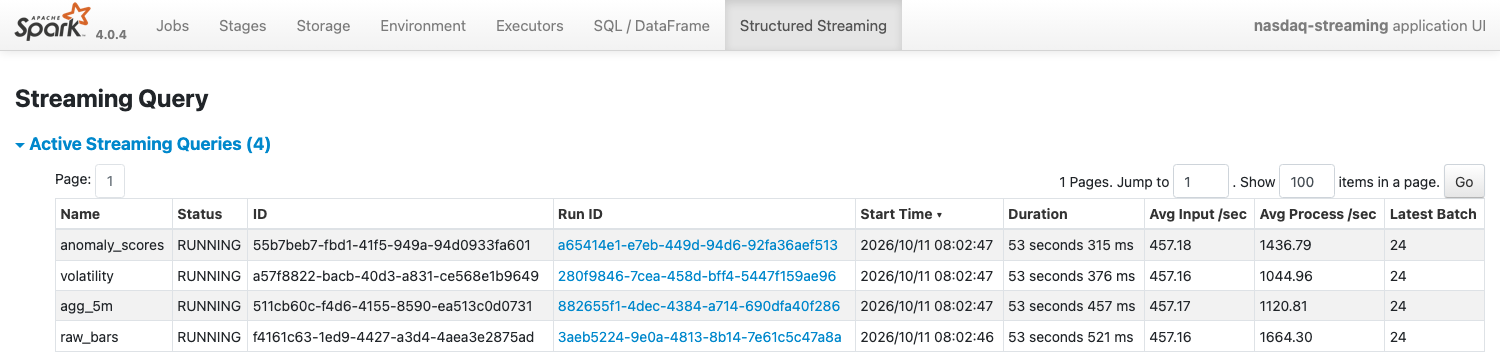
\includegraphics[width=\columnwidth]{fig_spark_queries.png}
\caption{Spark UI during the live run: four concurrent streaming queries with their input and processing rates.}
\label{fig:spark}
\end{figure}

\subsection{Resource Configuration}
Spark runs in local mode with a 3~GB driver heap, six shuffle partitions and a two-second processing-time trigger. The session pins the default Hadoop file system to the local disk and the time zone to UTC. Both settings were added in response to problems described in Section~IX.

\section{Machine Learning Implementation}

\subsection{Problem Formulation}
The aim is to flag one-minute bars whose behaviour is unusual for that company at that time of day. The target is a contextual anomaly in the sense of Chandola \emph{et al.}\ \cite{chandola2009}. No labelled anomalies exist for this data, so an unsupervised model is trained on the bars and evaluation is carried out on injected events (Section~VII-F).

\subsection{Feature Engineering}
Three raw quantities are derived from every bar: the log return $r=\ln(C/O)$, the relative range $g=(H-L)/O$ and the log volume $v=\ln(1+V)$. Each is standardised against a baseline computed per symbol and per half-hour bucket $b$ of the trading day:
\begin{equation}
z_x=\operatorname{clip}\!\left(\frac{x-\mu_{s,b}(x)}{\max\!\big(\sigma_{s,b}(x),\,10^{-6}\big)},\,-10,\,10\right),
\end{equation}
for $x\in\{r,g,v\}$ and symbol $s$. The feature vector is $(|z_r|,\,z_g,\,z_v)$. The absolute value is taken for the return because a large move in either direction is equally abnormal. The baseline has 650 rows, 50 symbols by 13 half-hour buckets, and was computed from the training sessions only. Clipping at $\pm10$ bounds the influence of the extreme tail on the cluster centres.

\subsection{Model}
The model is an MLlib \code{Pipeline} of a \code{VectorAssembler} and a \code{KMeans} stage with $k=4$, 50 iterations and a fixed seed. Because the training data contain the very anomalies the model should detect, a trimmed fit is used: a first model is trained, the 1\% of training bars farthest from their nearest centre are removed, and a second model is trained on the remainder. The anomaly score of a bar is its Euclidean distance to the nearest centre of the second model, and the decision threshold is the 99.5th percentile of the training scores, 3.388. Table~\ref{tab:centres} lists the centres. The clusters have a plain reading: a large cluster of quiet bars below baseline range and volume, a cluster of high-volume bars with ordinary movement, a cluster of larger moves with normal volume, and a small cluster that is elevated on all three features.

\begin{table}[t]
\caption{KMeans Cluster Centres and Share of the 135,028 Scored Bars}
\label{tab:centres}
\centering
\small
\begin{tabular}{@{}lrrrr@{}}
\toprule
Cluster & $|z_r|$ & $z_g$ & $z_v$ & Share \\
\midrule
1 (quiet) & 0.35 & $-0.72$ & $-0.83$ & 41.6\% \\
2 (high volume) & 0.47 & $-0.12$ & 0.71 & 27.3\% \\
0 (larger move) & 1.12 & 0.44 & $-0.09$ & 20.0\% \\
3 (active) & 1.88 & 1.86 & 1.19 & 11.2\% \\
\bottomrule
\end{tabular}
\end{table}

\subsection{Scoring Inside the Stream}
The baseline is loaded once as a static DataFrame and joined to the stream on symbol and bucket with a broadcast hint. The z-scores, the fitted pipeline and the distance computation are then ordinary column expressions, so scoring is stateless: it needs no per-key state store and restarts cleanly from checkpoints. The distance to the nearest centre is written as a Spark SQL expression over the centres' coordinates rather than as a Python function, which avoids serialising rows to a Python worker. A bar is flagged by KMeans when its score exceeds the threshold and by the baseline rule when $|z_r|>4$.

\subsection{Training Set and Hold-out}
The first six sessions (115,800 bars) form the training set and the final session (19,228 bars) is held out. On the training set the KMeans rule flags 0.49\% of bars and the baseline rule 0.32\%. On the held-out session the rates are 1.12\% and 0.48\%. The higher KMeans rate on the held-out session is almost entirely one symbol: 116 of its 215 flags are TMUS, whose price gapped down at the start of that session (Section~VIII-F). With TMUS excluded, the KMeans flag rate on the held-out session is 0.53\%, in line with the 0.49\% seen in training.

\subsection{Evaluation Protocol}
Because genuine anomalies are unlabelled, anomalies were injected into the held-out session with a fixed seed. Each bar was selected with probability 1\%, giving 196 injected bars. A selected bar received, with equal probability, a price shock, a volume surge or both. A price shock moves the close by between 3 and 12 standard deviations of that symbol's baseline return, in a random direction, with the high and low adjusted to contain it. A volume surge multiplies the volume by a factor between 3 and 10. Precision, recall and F1 are computed at each detector's fixed threshold, and the areas under the ROC and precision-recall curves are computed from the continuous scores, which does not depend on the threshold choice.

\section{Results and Visual Insights}

\subsection{Dashboard Overview}
Fig.~\ref{fig:dash} shows the complete dashboard for NVDA over the last three days. The top row holds five headline tiles. Below them are the candlestick chart with VWAP, a bar chart of the largest movers, a status grid of volatility by ticker, a volatility comparison, the anomaly overlay, a table of the latest anomalies and two pipeline-health series. A symbol selector re-targets the symbol-specific panels. Lines break at market-closed gaps so that an overnight move is not drawn as if it were a price path.

\begin{figure*}[t]
\centering
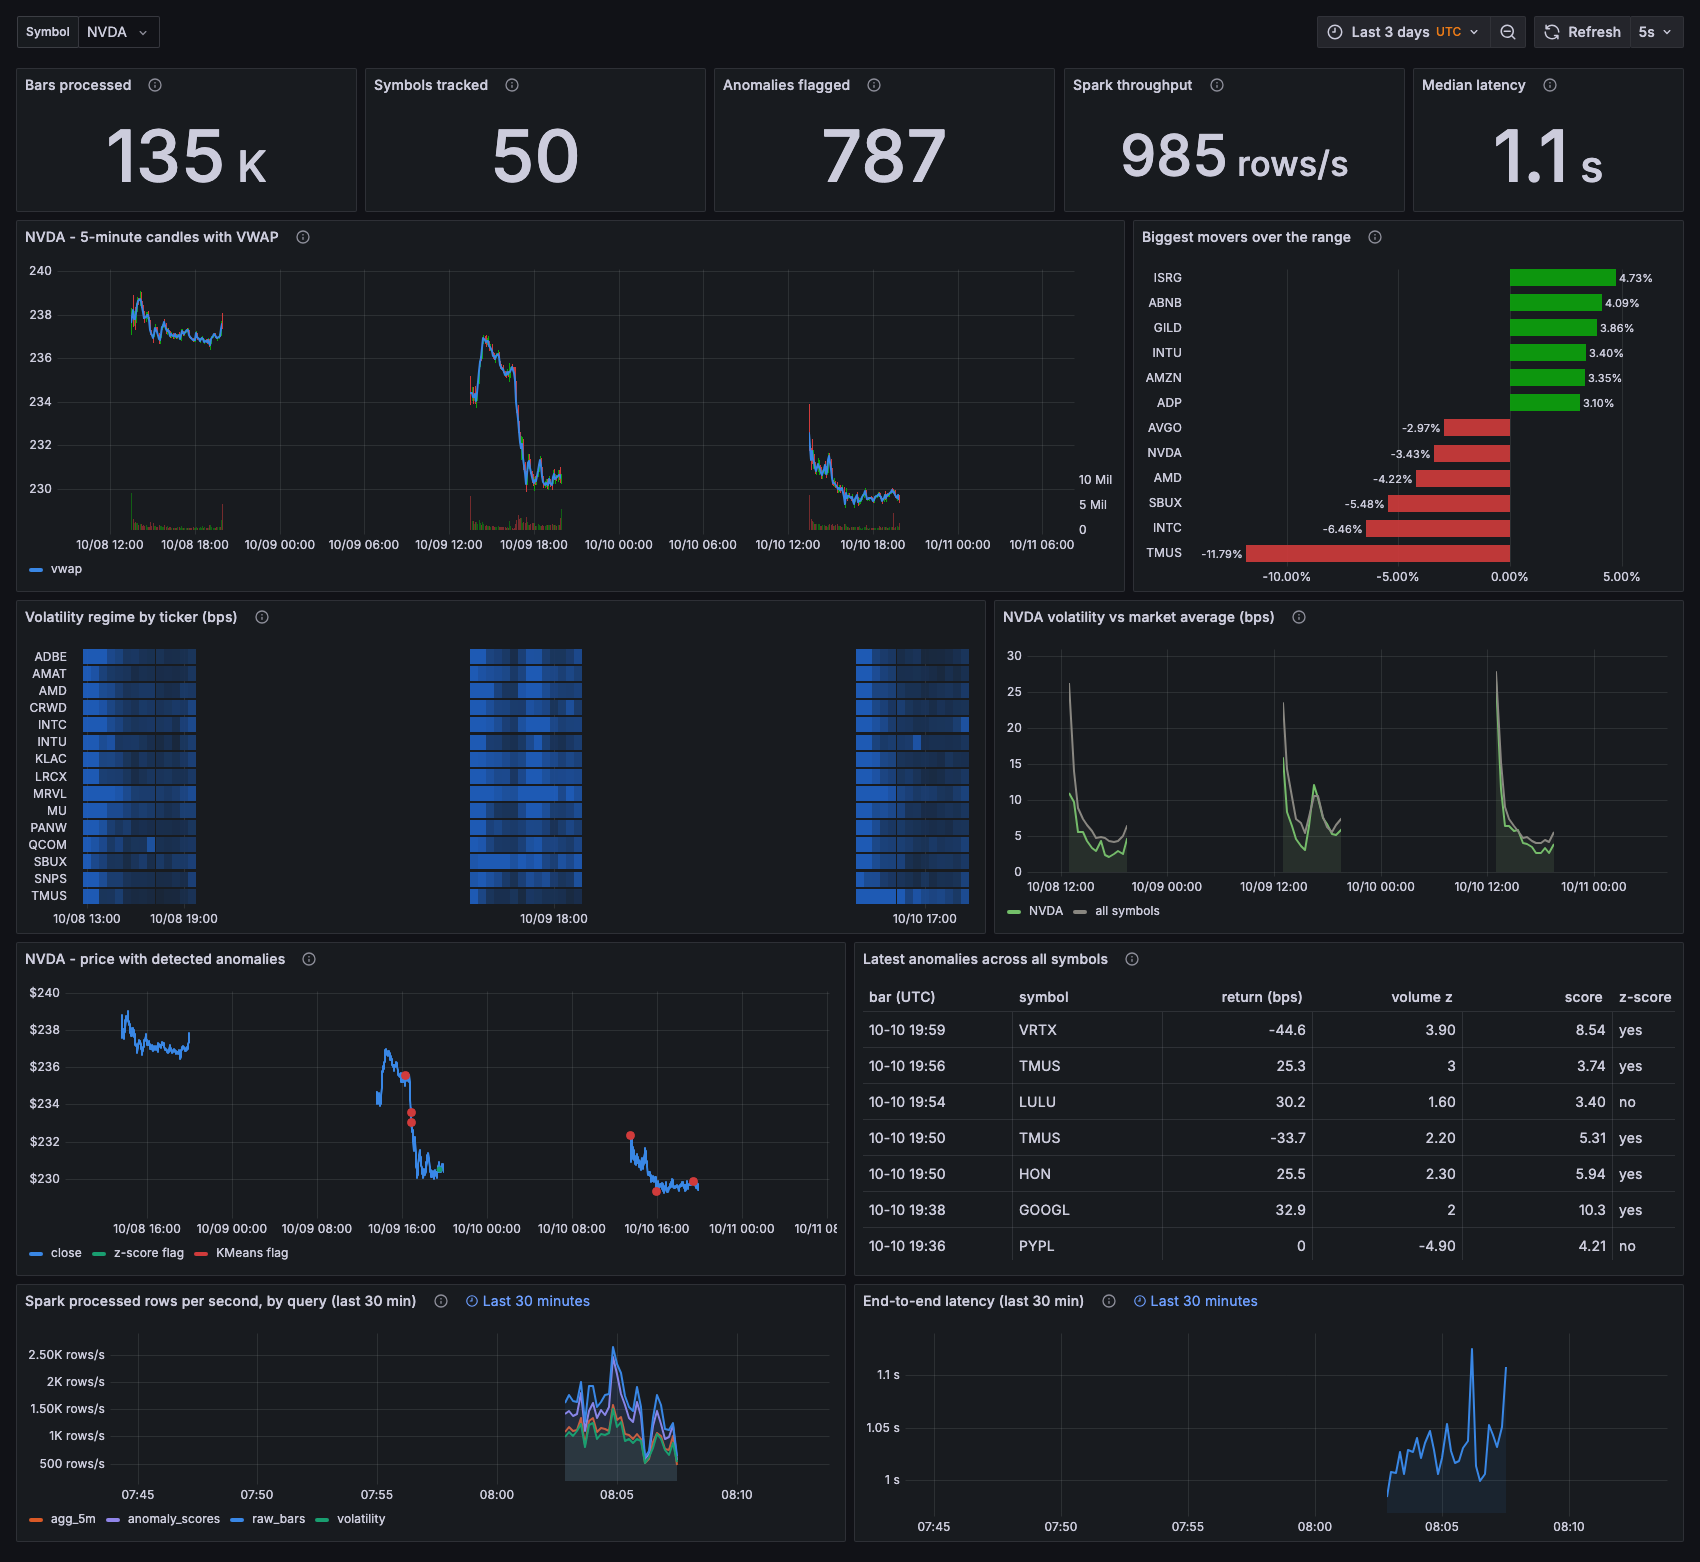
\includegraphics[width=0.86\textwidth]{grafana_dashboard.png}
\caption{The complete Grafana dashboard for NVDA, three-day range, taken after a live replay.}
\label{fig:dash}
\end{figure*}

\subsection{Headline Metrics}
Table~\ref{tab:headline} summarises the output of one complete replay. KMeans flagged 787 bars (0.58\%) and the baseline rule 465 (0.34\%). Of the baseline flags, 370 (80\%) were also flagged by KMeans. Of the 417 bars flagged only by KMeans, 264 (63\%) had a volume z-score of at least 3, which is the signature of an event that the return-only rule cannot see.

\begin{table}[t]
\caption{Headline Results of One Complete Replay}
\label{tab:headline}
\centering
\small
\begin{tabular}{@{}lr@{}}
\toprule
Metric & Value \\
\midrule
Bars processed & 135,028 \\
Symbols & 50 \\
Five-minute candles & 27,249 \\
Sliding volatility windows & 140,550 \\
KMeans anomaly flags & 787 (0.58\%) \\
Baseline z-score flags & 465 (0.34\%) \\
Flagged by both & 370 \\
Median 15-min volatility & 5.67 bps \\
Share of volume in first half-hour & 20.3\% \\
\bottomrule
\end{tabular}
\end{table}

\subsection{The Intraday Pattern}
Fig.~\ref{fig:intraday} confirms the intraday structure described in the literature \cite{admati1988}. The mean absolute one-minute return is 14.5 basis points in the opening half-hour and settles between 3.6 and 4.6 basis points through the middle of the day. Volume per bar is 76 thousand shares in the first half-hour, about 18 to 20 thousand at midday and 52 thousand in the last half-hour. The first half-hour alone carries 20.3\% of all volume. The KMeans flag rate is highest, at 1.06\%, in the opening half-hour, which is still near the 0.58\% overall rate rather than many times above it, as a raw threshold on price change would be. It is also elevated in the 11:30 and 12:00 half-hours (0.79\% and 0.81\%), the latter partly because of the market-wide event described below. Volatility peaks decay quickly in every session, as the NVDA series against the market average shows in Fig.~\ref{fig:volmarket}.

\begin{figure*}[t]
\centering
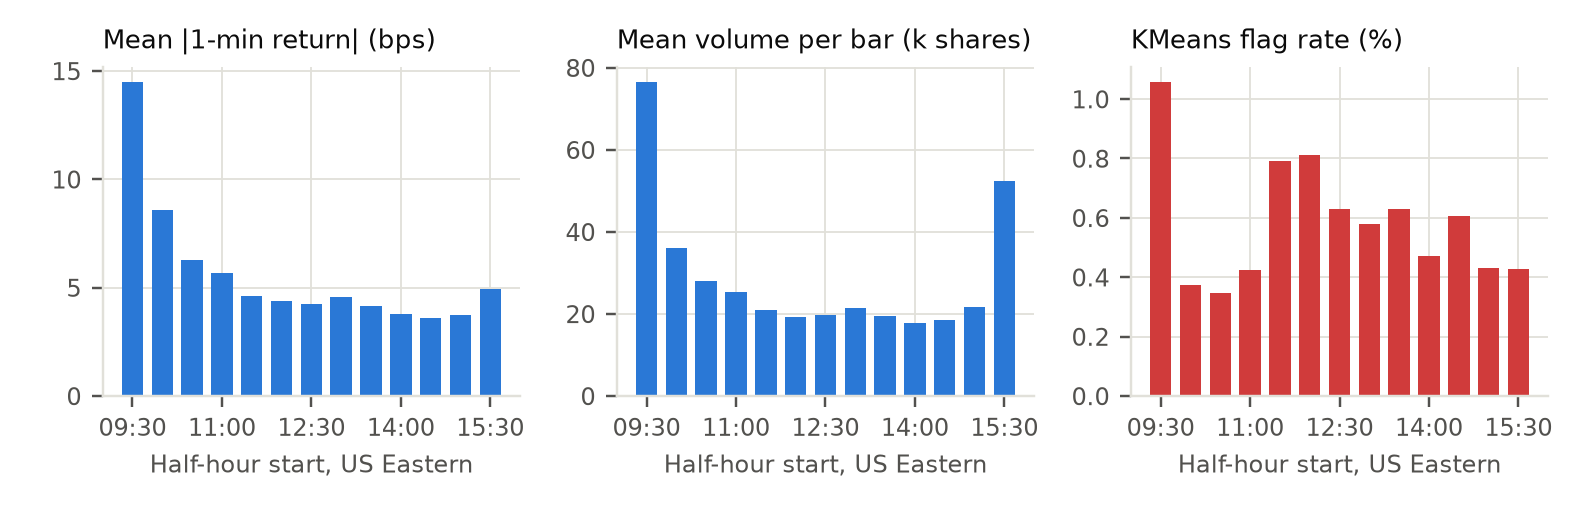
\includegraphics[width=0.92\textwidth]{chart_intraday.png}
\caption{Intraday profile over all 135,028 bars by half-hour of the trading day (US Eastern): mean absolute return, mean volume per bar and KMeans flag rate.}
\label{fig:intraday}
\end{figure*}

\begin{figure}[t]
\centering
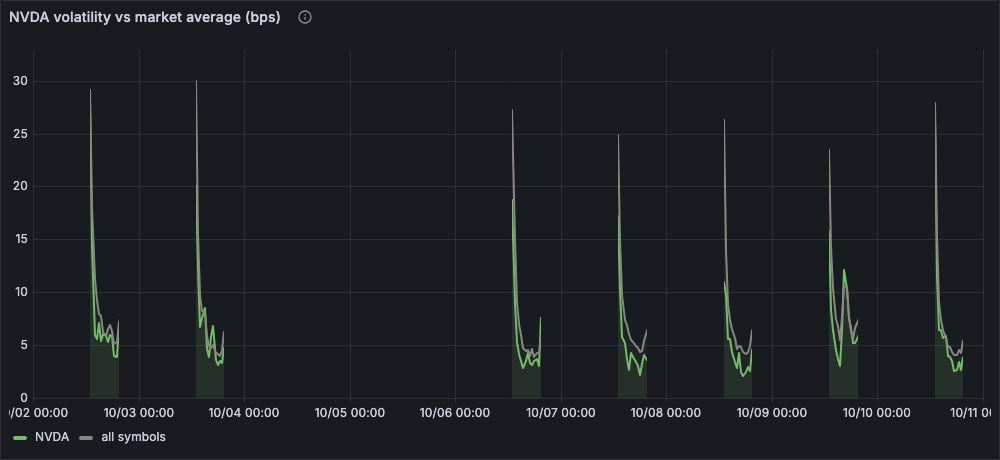
\includegraphics[width=\columnwidth]{panel_volatility_vs_market.png}
\caption{NVDA fifteen-minute return volatility against the average of all fifty symbols across the seven sessions, in basis points.}
\label{fig:volmarket}
\end{figure}

\subsection{Price Action and Movers}
Fig.~\ref{fig:candles} shows NVDA through the final session. The price opens with a sharp range in the first minutes, drifts downward through the morning and then trades in a narrow band around its VWAP for the afternoon, with candle bodies shrinking as volume falls. Over the whole week the largest gains, measured from the first five-minute open to the last closed five-minute window, were CSCO (+9.65\%), MELI (+9.26\%) and SNPS (+8.84\%), and the largest losses were INTC ($-11.76$\%) and TMUS ($-9.30$\%) (Fig.~\ref{fig:movers}).

\begin{figure*}[t]
\centering
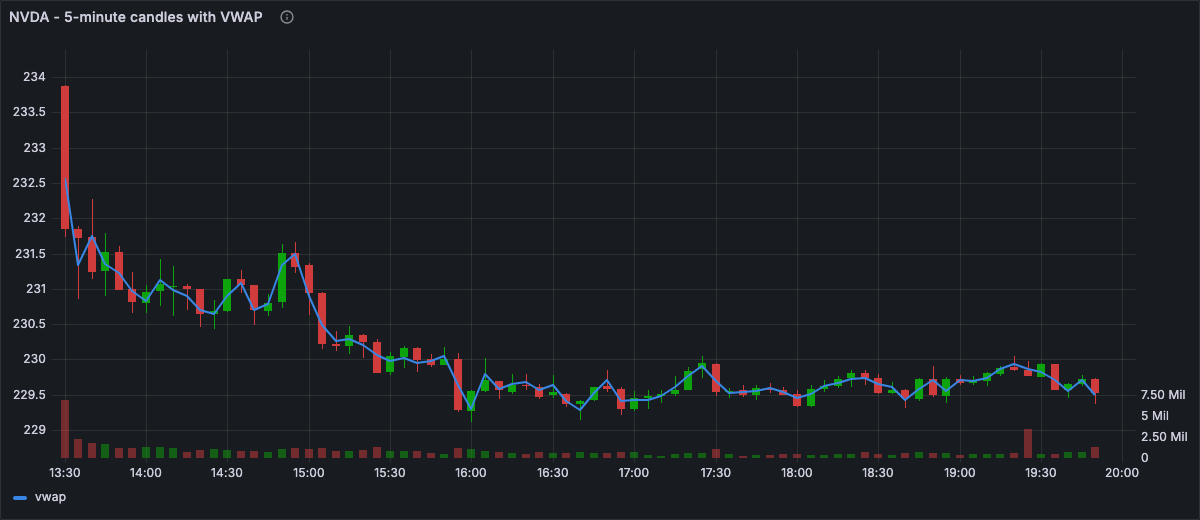
\includegraphics[width=0.82\textwidth]{panel_candles_nvda.png}
\caption{NVDA five-minute candles with VWAP and volume for the final session. Green candles close above their open and red below.}
\label{fig:candles}
\end{figure*}

\begin{figure}[t]
\centering
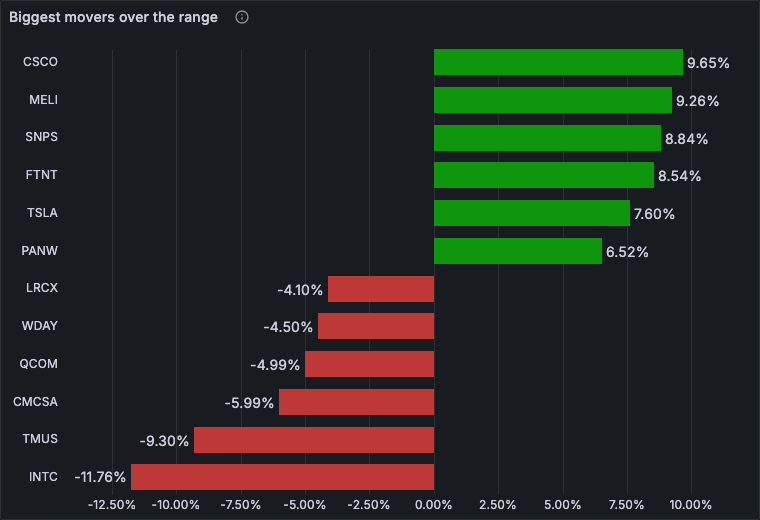
\includegraphics[width=0.9\columnwidth]{panel_movers.png}
\caption{Six largest gains and six largest losses over the week.}
\label{fig:movers}
\end{figure}

\subsection{Volatility Regimes}
The median fifteen-minute volatility across all windows is 5.67 basis points. The most volatile names by mean window volatility are MRVL (16.2 bps), SNPS (11.2), INTC (11.1), MU (10.6) and LRCX (10.1), predominantly semiconductor and software-tool companies, and the least volatile are ADP (4.6), CSX (4.2) and COST (4.1). Fig.~\ref{fig:heat} shows the regime grid for the fifteen most volatile tickers during the final session. The brightest column is the opening half-hour for every name, which is the common market-wide component of volatility, while rows that stay brighter through the day belong to the structurally more volatile names.

\begin{figure}[t]
\centering
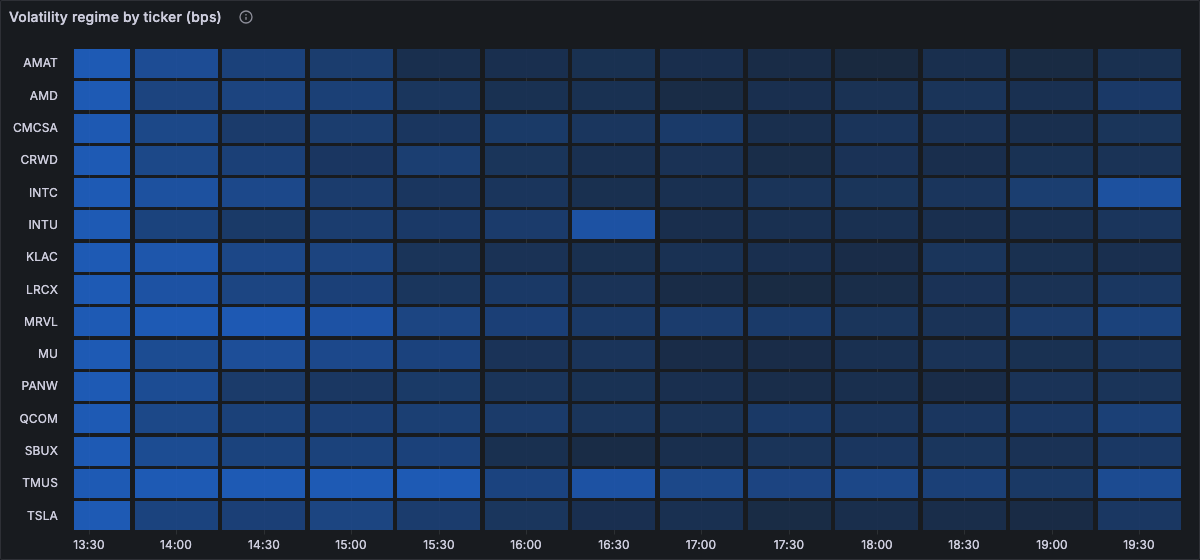
\includegraphics[width=\columnwidth]{panel_volatility_heatmap.png}
\caption{Mean fifteen-minute volatility by ticker and half-hour for the fifteen most volatile symbols, final session.}
\label{fig:heat}
\end{figure}

\subsection{Anomalies}
The model separates a dense core of ordinary bars from a long tail of abnormal ones (Fig.~\ref{fig:hist}). Two findings stand out.

\emph{A market-wide event.} At 16:17 UTC (12:17 US Eastern) on source day 8 October, 36 of the 50 symbols were flagged within the same minute, by far the largest simultaneous cluster in the data. The next largest clusters, of 10 to 16 symbols, fell mostly in session-opening minutes. A simultaneous cluster across unrelated companies points to a market-wide cause such as a macroeconomic release rather than a company event, although the data themselves cannot identify the cause.

\emph{A regime shift is flagged repeatedly.} TMUS accounts for 129 of the 787 flags, 16\% of the total. Fig.~\ref{fig:tmus} shows why. Its price gapped down by about 9\% between the close of one session and the next open, from about \$171 to about \$155, and then traded around that new level. The static baseline still describes the old regime, so most bars of the following session look unusual relative to it. This is a correct reading of the baseline and also a limitation of the design: after a lasting level change, a static baseline keeps raising alarms that no longer carry information. Section~X-D returns to this.

\begin{figure}[t]
\centering
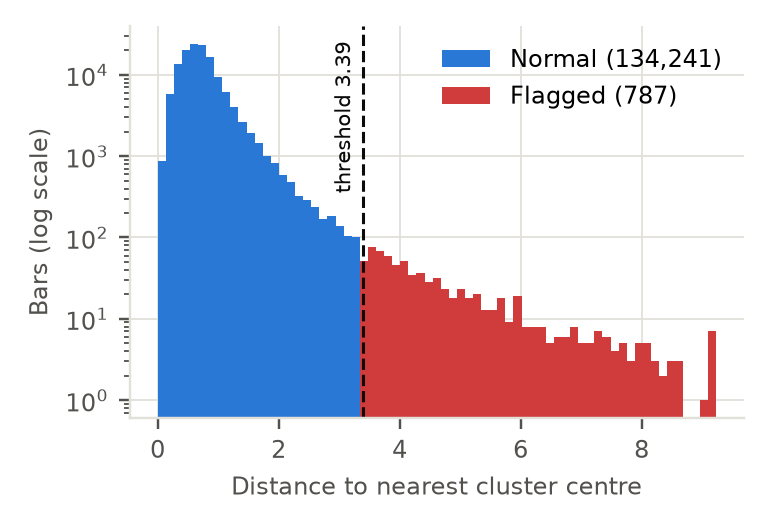
\includegraphics[width=\columnwidth]{chart_score_hist.png}
\caption{Distribution of the KMeans anomaly score on a logarithmic count axis, with the 99.5th-percentile threshold.}
\label{fig:hist}
\end{figure}

\begin{figure*}[t]
\centering
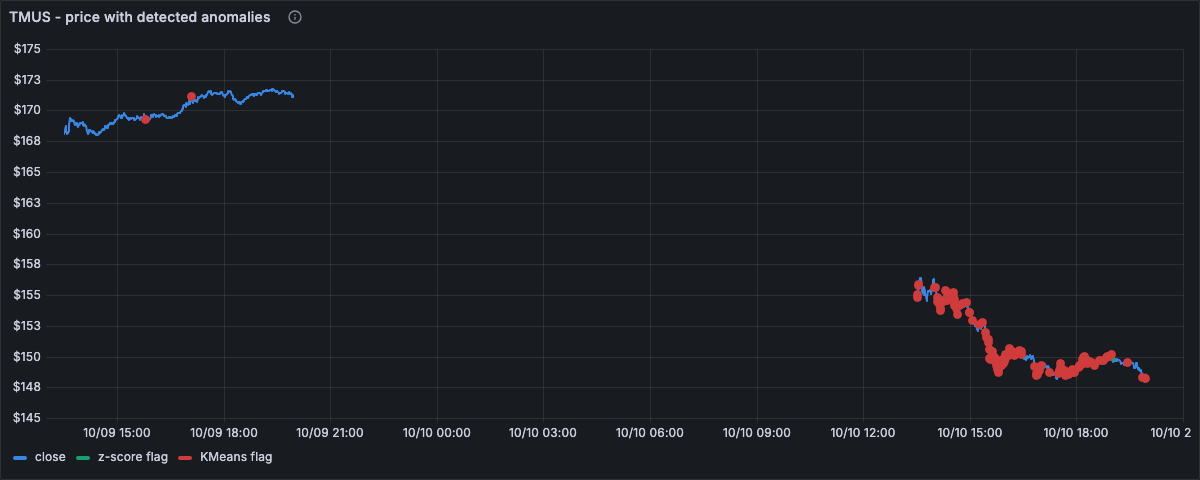
\includegraphics[width=0.82\textwidth]{panel_anomalies_tmus.png}
\caption{TMUS price with KMeans flags (red) over the last two sessions. The gap between sessions is left blank by the dashboard.}
\label{fig:tmus}
\end{figure*}

\subsection{Detection Quality}
Table~\ref{tab:eval} and Fig.~\ref{fig:eval} give the results on the held-out session with injected anomalies. KMeans has the higher recall (0.69 against 0.64) and a clearly better ranking, with an area under the ROC curve of 0.968 against 0.862. At the fixed thresholds, however, the baseline has the higher precision (0.58 against 0.39) and the higher F1 (0.61 against 0.50). Two facts explain this. First, the held-out session contains the TMUS regime shift: 116 of the 215 bars that KMeans flags in that session belong to that one symbol, so the model's false positive rate there is 1.12\% against 0.49\% on the training sessions, and most of the excess is traceable to a single stock. Second, the baseline cannot see nearly a third of the injected events (58 of 196 are volume-only). Its recall on volume-only surges is zero, while KMeans catches 12\% of them. Even KMeans recovers only a small fraction of volume surges, because a volume multiple of three to ten applied to a bar that was already at the baseline moves it only moderately far in the clipped log-volume feature. The model's value is therefore real but limited, and it is best read as a ranking tool: an analyst reviewing the top-scored bars sees the genuine events earlier than with the return rule.

\begin{table}[t]
\caption{Detector Results on the Held-out Session (196 Injected Anomalies in 19,228 Bars)}
\label{tab:eval}
\centering
\small
\begin{tabular}{@{}lrr@{}}
\toprule
Metric & KMeans & Return z-score \\
\midrule
Precision & 0.389 & 0.575 \\
Recall & 0.694 & 0.643 \\
F1 & 0.498 & 0.607 \\
AUC-ROC & 0.968 & 0.862 \\
AUC-PR & 0.630 & 0.620 \\
False positive rate & 1.12\% & 0.49\% \\
Recall, price shock & 0.913 & 0.899 \\
Recall, volume surge & 0.121 & 0.000 \\
Recall, both & 0.957 & 0.928 \\
True / false positives & 136 / 214 & 126 / 93 \\
\bottomrule
\end{tabular}
\end{table}

\begin{figure*}[t]
\centering
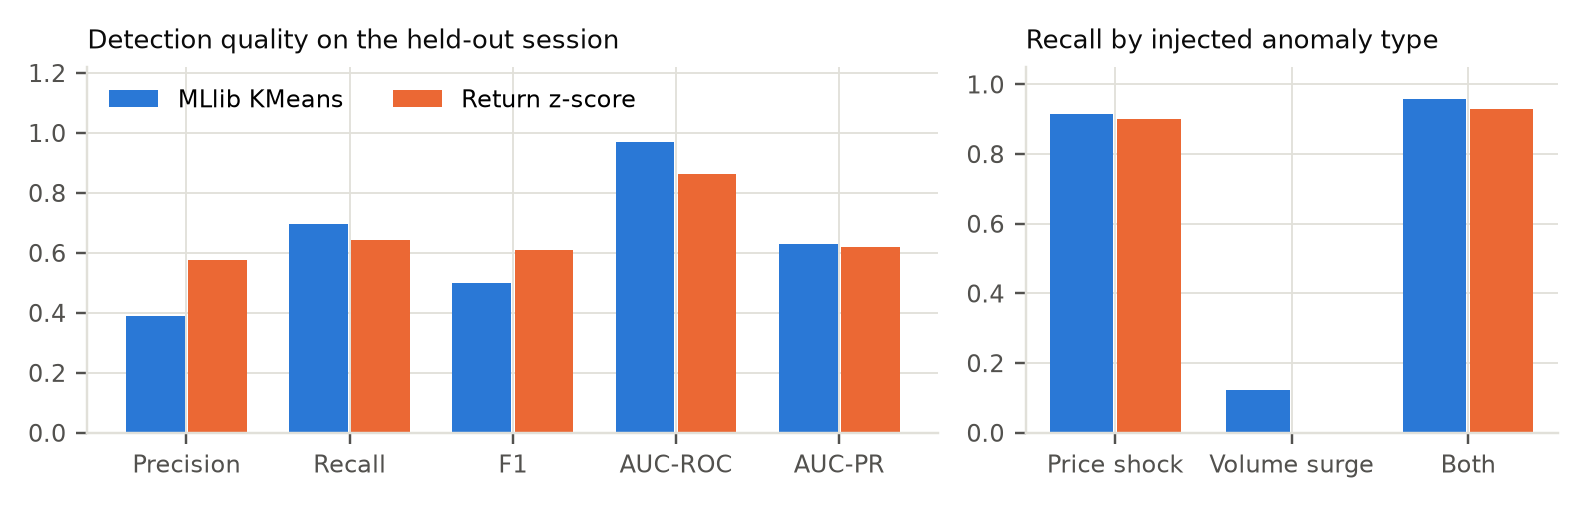
\includegraphics[width=0.9\textwidth]{chart_evaluation.png}
\caption{Detector comparison on the held-out session: overall metrics (left) and recall by injected anomaly type (right).}
\label{fig:eval}
\end{figure*}

\subsection{Pipeline Performance}
Table~\ref{tab:perf} reports the per-query throughput recorded by the listener during the live replay at $600\times$, in which about 500 messages per second were produced. Each of the four queries consumed all 135,028 rows. The raw-bar query, which only parses and writes, processed 1,601 rows per second on average with a mean micro-batch of 0.7~s. The windowed and model-scoring queries were slower, as expected, because they hold state or perform a join. The median produce-to-process latency was 1.03~s, the 95th percentile 1.93~s and the maximum 2.39~s, against the target of five seconds. When the whole backlog was instead loaded first and drained with all four queries running concurrently, 135,028 rows per query were processed in about 40~s including Spark start-up, which shows that the pipeline can run well above the replay rate. Fig.~\ref{fig:health} shows the two health panels from the live run.

\begin{table}[t]
\caption{Throughput per Streaming Query During the Live Replay}
\label{tab:perf}
\centering
\footnotesize
\setlength{\tabcolsep}{3pt}
\begin{tabular}{@{}lrrrr@{}}
\toprule
Query & Batches & Mean rows/s & Peak rows/s & Batch ms \\
\midrule
\code{raw\_bars} & 142 & 1,601 & 3,556 & 715 \\
\code{anomaly\_scores} & 142 & 1,385 & 3,432 & 814 \\
\code{agg\_5m} & 142 & 1,039 & 1,881 & 1,033 \\
\code{volatility} & 141 & 975 & 1,741 & 1,115 \\
\bottomrule
\end{tabular}
\end{table}

\begin{figure*}[t]
\centering
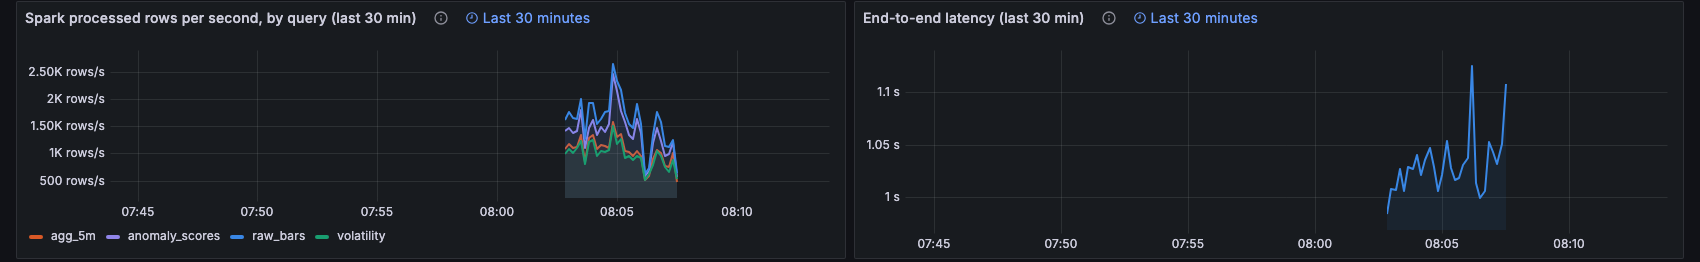
\includegraphics[width=0.9\textwidth]{panel_pipeline_health.png}
\caption{Pipeline-health panels from the live replay: processed rows per second by query (left) and produce-to-process latency (right).}
\label{fig:health}
\end{figure*}

\section{Testing and Evaluation}

Table~\ref{tab:tests} lists the verification activities. Each was run against the real system and its observed result is the one reported.

\begin{table*}[t]
\caption{Test Cases and Outcomes}
\label{tab:tests}
\centering
\small
\begin{tabular}{@{}llp{3.7cm}p{6.8cm}l@{}}
\toprule
ID & Component & Test objective & Observed result & Status \\
\midrule
T1 & Dataset & Rows, nulls, duplicates, price relations & 135,028 rows, 0 nulls, 0 duplicates, 0 OHLC violations & Passed \\
T2 & Kafka & Topic created with partitions & \code{ticks.raw} with 3 partitions, replication factor 1 & Passed \\
T3 & Kafka & Console consumer read-back & JSON bars read back from the topic & Passed \\
T4 & Producer & Unthrottled replay of the full set & 135,028 sent, 135,028 delivered, 0 failed in 1.4~s & Passed \\
T5 & Spark & Drain backlog through four queries & Each query consumed 135,028 rows & Passed \\
T6 & Sink & Row counts in PostgreSQL & 135,028 bars and scores, 27,249 candles, 140,550 windows & Passed \\
T7 & Candles & Compare with pandas, all windows & 27,249 of 27,249 matched; difference 0 for OHLC, volume and count; VWAP within $5\times10^{-13}$ & Passed \\
T8 & Volatility & Compare with pandas, 2,000 sampled windows & Maximum difference $9\times10^{-19}$; bar counts equal & Passed \\
T9 & Watermark & Windows not yet closed & 50 final windows, one per symbol, not emitted & Passed (expected) \\
T10 & Checkpoint & Re-run job with existing checkpoints & No new rows; all counts unchanged & Passed \\
T11 & Latency & Live replay at $600\times$ & Median 1.03~s, p95 1.93~s, max 2.39~s & Passed (target 5~s) \\
T12 & Model & Held-out evaluation with injection & AUC-ROC 0.968, F1 0.498 (Table~\ref{tab:eval}) & Reported \\
T13 & Grafana & Execute all 13 panel queries via API & 0 errors & Passed \\
T14 & Dashboard & Render panels and inspect & Defects found and fixed (Section~IX-A) & Passed after fix \\
\bottomrule
\end{tabular}
\end{table*}

\subsection{Issues Encountered}
Several defects were met and resolved; they are recorded because each changed the final configuration.
\begin{enumerate}
\item \emph{Spark resolved local paths against HDFS.} A Hadoop installation on the development machine set \code{HADOOP\_CONF\_DIR}, so Spark read the scheme-less Parquet path from \code{hdfs://localhost:9000} and failed with a connection refusal. The session now sets \code{spark.hadoop.fs.defaultFS} to \code{file:///}.
\item \emph{PostgreSQL port conflict.} A PostgreSQL instance was already listening on 5432, so the container did not start. The container is published on host port 5433.
\item \emph{Download cache lock.} The multi-threaded download intermittently lost one symbol to a lock on the library's SQLite time-zone cache. Missing symbols are now retried sequentially and the cache is kept inside the project's data directory.
\item \emph{Single-precision noise in prices.} Prices such as 245.3699951171875 appeared in Kafka. They are rounded to four decimals at download time.
\item \emph{A column named \code{time} must be a timestamp.} The anomaly table in Grafana failed because a text column carried that name; it was renamed.
\item \emph{Lines crossing market-closed gaps.} Setting \code{spanNulls} did not break the lines across the overnight gap; the separate \code{insertNulls} option did.
\item \emph{Noisy shutdown.} In drain mode the Python listener raised errors when the JVM exited. The listener is now removed and the session stopped explicitly.
\item \emph{Latency wording.} The first dashboard text described the measurement as time to ``written to PostgreSQL''. The processed time is taken when the micro-batch starts, just before the write, and the description was corrected to ``produce-to-process''.
\end{enumerate}

\section{Discussion}

\subsection{How the Work Meets the Problem}
The pipeline ingests a stream of bars, produces event-time aggregates and an anomaly score within about a second, stores them and displays them. The windowed results were verified against an independent computation and match exactly, so the dashboard's numbers can be trusted as faithful functions of the data. The model's behaviour was evaluated on labelled injected events rather than asserted.

\subsection{Alignment with the Evaluation Criteria}
Table~\ref{tab:criteria} relates the work to the CA-3 rubric.

\begin{table}[t]
\caption{Mapping of the Project to the Evaluation Criteria}
\label{tab:criteria}
\centering
\small
\begin{tabular}{@{}p{2.4cm}p{5.4cm}@{}}
\toprule
Criterion & Where it is addressed \\
\midrule
Problem identification & Sections I and II: stated problem, objectives, Big Data rationale (velocity, volume, variety of tick data) \\
Tool and framework usage & Sections III, V, VI, VII: Kafka, Spark Structured Streaming, MLlib, PostgreSQL and Grafana, each with a stated rationale \\
Data processing and analysis & Sections IV, VI, VII, IX: validated data, event-time windows with watermarks, KMeans scoring, cross-checks \\
Visualisation and insights & Section VIII: thirteen-panel Grafana dashboard and interpreted findings \\
Innovation and real-world relevance & Sections VII and X: context-normalised stateless scoring in the stream, injected-anomaly evaluation, surveillance use \\
Report & Whole report: IEEE format, evidence-based, referenced \\
\bottomrule
\end{tabular}
\end{table}

\subsection{Practical Relevance}
The same structure, a log, a streaming engine, a scoring model and a SQL-backed dashboard, serves market surveillance, intraday risk monitoring and operations dashboards for trading platforms. A context-normalised flag is more useful to an analyst than a raw threshold on price change, because it already accounts for the symbol's character and the time of day. Persisting the z-scores beside each flag lets a reviewer see why a bar was marked. The system is a monitoring aid: it ranks bars for attention and does not issue trading advice.

\subsection{Limitations}
The following limitations should be considered when interpreting the results.
\begin{enumerate}
\item The feed is a replay of one week of historical bars, not a live exchange connection, so latency describes the pipeline and not market data delivery.
\item The data volume (135,028 bars) is modest. The replay speed and the unthrottled drain were used to exercise the system, but no multi-day, multi-node or fault-injection test was performed.
\item Spark runs in local mode on one machine, Kafka has one broker and one replica, and PostgreSQL is a single instance. No scalability or high-availability claim is made.
\item The sink gives at-least-once delivery. Only a clean restart was tested.
\item Anomaly evaluation relies on injected events. Real anomalies may differ in shape and are unlabelled.
\item The baseline is static. After a lasting level change, as in the TMUS case, the model keeps flagging bars until it is retrained.
\item The held-out session contained a lasting level change in one symbol (TMUS), which accounts for most of the KMeans false positives there; the threshold is not recalibrated online.
\item Only three features and four clusters were used, and neither was tuned beyond a single fit.
\item Bars are one-minute summaries; sub-minute events are invisible to the system.
\end{enumerate}

\section{Conclusion and Future Work}
This project built and documented a real-time analytics pipeline for NASDAQ equities. One week of one-minute bars for 50 symbols was replayed through Kafka, processed by four concurrent Spark Structured Streaming queries, scored by an MLlib KMeans anomaly model, stored in PostgreSQL and presented on a Grafana dashboard. The streaming aggregates match an independent computation exactly, the pipeline delivered a median latency of about one second at six hundred times real time, and the anomaly model ranked injected events substantially better than a return-only rule while remaining weaker at a fixed threshold. The study also showed where the design is thin: the baseline is static, the sink is at-least-once and the evaluation uses injected events.

Future work could add the following: an idempotent upsert sink keyed on symbol and window; a rolling or daily-refreshed baseline so that regime shifts stop raising alarms; online threshold calibration; additional features such as cross-sectional return relative to the index; a live market-data connection; and a multi-broker Kafka and multi-executor Spark deployment to measure scaling. These are proposals and are not part of the implemented system.

\section*{Acknowledgment}
The author thanks the course faculty and the department for guidance and for access to the laboratory and software environment.

\begin{thebibliography}{99}
\bibitem{kreps2011} J. Kreps, N. Narkhede, and J. Rao, ``Kafka: A distributed messaging system for log processing,'' in \emph{Proc. 6th Int. Workshop Netw. Meets Databases (NetDB)}, Athens, Greece, 2011.
\bibitem{zaharia2010} M. Zaharia, M. Chowdhury, M. J. Franklin, S. Shenker, and I. Stoica, ``Spark: Cluster computing with working sets,'' in \emph{Proc. 2nd USENIX Workshop Hot Topics Cloud Comput. (HotCloud)}, Boston, MA, USA, 2010.
\bibitem{zaharia2012} M. Zaharia \emph{et al.}, ``Resilient distributed datasets: A fault-tolerant abstraction for in-memory cluster computing,'' in \emph{Proc. 9th USENIX Symp. Networked Syst. Design Implement. (NSDI)}, San Jose, CA, USA, 2012, pp. 15--28.
\bibitem{armbrust2018} M. Armbrust \emph{et al.}, ``Structured Streaming: A declarative API for real-time applications in Apache Spark,'' in \emph{Proc. Int. Conf. Manage. Data (SIGMOD)}, Houston, TX, USA, 2018, pp. 601--613.
\bibitem{meng2016} X. Meng \emph{et al.}, ``MLlib: Machine learning in Apache Spark,'' \emph{J. Mach. Learn. Res.}, vol. 17, no. 34, pp. 1--7, 2016.
\bibitem{akidau2015} T. Akidau \emph{et al.}, ``The dataflow model: A practical approach to balancing correctness, latency, and cost in massive-scale, unbounded, out-of-order data processing,'' \emph{Proc. VLDB Endow.}, vol. 8, no. 12, pp. 1792--1803, Aug. 2015.
\bibitem{chandola2009} V. Chandola, A. Banerjee, and V. Kumar, ``Anomaly detection: A survey,'' \emph{ACM Comput. Surv.}, vol. 41, no. 3, pp. 15:1--15:58, Jul. 2009.
\bibitem{lloyd1982} S. P. Lloyd, ``Least squares quantization in PCM,'' \emph{IEEE Trans. Inf. Theory}, vol. 28, no. 2, pp. 129--137, Mar. 1982.
\bibitem{arthur2007} D. Arthur and S. Vassilvitskii, ``k-means++: The advantages of careful seeding,'' in \emph{Proc. 18th Annu. ACM-SIAM Symp. Discrete Algorithms (SODA)}, New Orleans, LA, USA, 2007, pp. 1027--1035.
\bibitem{bahmani2012} B. Bahmani, B. Moseley, A. Vattani, R. Kumar, and S. Vassilvitskii, ``Scalable k-means++,'' \emph{Proc. VLDB Endow.}, vol. 5, no. 7, pp. 622--633, Mar. 2012.
\bibitem{admati1988} A. R. Admati and P. Pfleiderer, ``A theory of intraday patterns: Volume and price variability,'' \emph{Rev. Financial Stud.}, vol. 1, no. 1, pp. 3--40, 1988.
\bibitem{carbone2015} P. Carbone, A. Katsifodimos, S. Ewen, V. Markl, S. Haridi, and K. Tzoumas, ``Apache Flink: Stream and batch processing in a single engine,'' \emph{IEEE Data Eng. Bull.}, vol. 38, no. 4, pp. 28--38, 2015.
\bibitem{kleppmann2017} M. Kleppmann, \emph{Designing Data-Intensive Applications}. Sebastopol, CA, USA: O'Reilly Media, 2017.
\bibitem{kip500} Apache Software Foundation, ``KIP-500: Replace ZooKeeper with a self-managed metadata quorum.'' [Online]. Available: \url{https://cwiki.apache.org/confluence/display/KAFKA/KIP-500}. Accessed: Oct. 2026.
\bibitem{pgdocs} PostgreSQL Global Development Group, ``PostgreSQL 16 documentation.'' [Online]. Available: \url{https://www.postgresql.org/docs/16/}. Accessed: Oct. 2026.
\bibitem{grafanadocs} Grafana Labs, ``Grafana documentation.'' [Online]. Available: \url{https://grafana.com/docs/grafana/latest/}. Accessed: Oct. 2026.
\bibitem{yfinance} R. Aroussi, ``yfinance: Download market data from Yahoo! Finance's API.'' [Online]. Available: \url{https://github.com/ranaroussi/yfinance}. Accessed: Oct. 2026.
\end{thebibliography}

\appendices

\section{Key Implementation Excerpts}

The five-minute candle aggregation (\code{streaming/transforms.py}):
\begin{lstlisting}
candles = (
    bars.withWatermark("bar_time", "2 minutes")
    .groupBy(F.window("bar_time", "5 minutes"), "symbol")
    .agg(
        F.min_by("open", "bar_time").alias("open"),
        F.max("high").alias("high"),
        F.min("low").alias("low"),
        F.max_by("close", "bar_time").alias("close"),
        F.sum("volume").alias("volume"),
        F.try_divide(
            F.sum(typical_price * F.col("volume")),
            F.sum("volume"),
        ).alias("vwap"),
        F.count("*").alias("bar_count"),
    )
)
\end{lstlisting}

Distance to the nearest centre and scoring (\code{ml/model.py}):
\begin{lstlisting}
def distance_to_nearest_center(features, centers):
    values = vector_to_array(F.col(features))
    distances = []
    for center in centers:
        squares = [
            (values[i] - F.lit(c)) ** 2
            for i, c in enumerate(center)
        ]
        distances.append(F.sqrt(reduce(add, squares)))
    return F.least(*distances)


def score_bars(bars, model):
    features = add_zscores(
        bars, model.baseline, model.z_clip
    )
    return (
        model.pipeline.transform(features)
        .withColumn(
            "kmeans_score",
            distance_to_nearest_center(
                "features", model.centers
            ),
        )
        .withColumn(
            "kmeans_anomaly",
            F.col("kmeans_score") > F.lit(model.threshold),
        )
        .withColumn(
            "zscore_anomaly",
            F.col("abs_z_return") > F.lit(model.z_threshold),
        )
    )
\end{lstlisting}

\section{Reproduction Commands}
\begin{lstlisting}[language=bash]
make venv        # virtual environment, dependencies
make up          # Kafka, PostgreSQL, Grafana, Kafka UI
make download    # 1-minute bars to Parquet
make train       # MLlib KMeans, one-day hold-out
make evaluate    # injected-anomaly evaluation
make stream      # terminal 1: Spark job
make produce SPEED=600   # terminal 2: replay
make reset       # clear checkpoints, tables, topic
\end{lstlisting}
Grafana is then available at \url{http://localhost:3000}, Kafka UI at \url{http://localhost:8080} and the Spark UI at \url{http://localhost:4040} while the job runs.

\section{Symbol Universe}
AAPL, MSFT, NVDA, AMZN, GOOGL, META, TSLA, AVGO, COST, NFLX, AMD, ADBE, PEP, CSCO, TMUS, INTC, CMCSA, QCOM, TXN, AMGN, INTU, HON, AMAT, SBUX, BKNG, ISRG, GILD, ADI, MDLZ, VRTX, REGN, LRCX, PANW, MU, KLAC, SNPS, CDNS, MELI, ASML, CRWD, ABNB, MAR, ORLY, FTNT, ADP, CSX, MRVL, PYPL, LULU, WDAY.

\end{document}
